\documentclass[14pt]{beamer}
\usepackage{./Estilos/BeamerUVM}
\usepackage{./Estilos/ColoresLatex}
%Sección para el tema de beamer, con el theme, usercolortheme y sección de footers
\usetheme{CambridgeUS}
\usecolortheme{wolverine}
%\useoutertheme{default}
\setbeamercovered{invisible}
% or whatever (possibly just delete it)
\setbeamertemplate{section in toc}[sections numbered]
\setbeamertemplate{subsection in toc}[subsections numbered]
\setbeamertemplate{subsection in toc}{\leavevmode\leftskip=3.2em\rlap{\hskip-2em\inserttocsectionnumber.\inserttocsubsectionnumber}\inserttocsubsection\par}
%\setbeamercolor{section in toc}{fg=blue}
%\setbeamercolor{subsection in toc}{fg=blue}
%\setbeamercolor{frametitle}{fg=blue}
\setbeamertemplate{caption}[numbered]

\setbeamertemplate{footline}
\beamertemplatenavigationsymbolsempty
\setbeamertemplate{headline}{}


\makeatletter
\setbeamercolor{secºtion in foot}{bg=gray!30, fg=black!90!orange}
\setbeamercolor{subsection in foot}{bg=blue!30!yellow, fg=red}
\setbeamercolor{date in foot}{bg=black, fg=white}
\setbeamertemplate{footline}
{
  \leavevmode%
  \hbox{%
  \begin{beamercolorbox}[wd=.333333\paperwidth,ht=2.25ex,dp=1ex,center]{section in foot}%
    \usebeamerfont{section in foot} \insertsection
  \end{beamercolorbox}%
  \begin{beamercolorbox}[wd=.333333\paperwidth,ht=2.25ex,dp=1ex,center]{subsection in foot}%
    \usebeamerfont{subsection in foot}  \insertsubsection
  \end{beamercolorbox}%
  \begin{beamercolorbox}[wd=.333333\paperwidth,ht=2.25ex,dp=1ex,right]{date in head/foot}%
    \usebeamerfont{date in head/foot} \insertshortdate{} \hspace*{2em}
    \insertframenumber{} / \inserttotalframenumber \hspace*{2ex} 
  \end{beamercolorbox}}%
  \vskip0pt%
}






% \usefonttheme{serif}
\usepackage[clock]{ifsym}
\DeclareSIUnit\erg{erg}
\DeclareSIUnit[number-unit-product = {\,}]\cal{cal}

\sisetup{per-mode=symbol}
\resetcounteronoverlays{saveenumi}

% Macro para agregar el logo de UVM en cada slide de la presentación

\addtobeamertemplate{frametitle}{}{%
\begin{tikzpicture}[remember picture,overlay]
\coordinate (logo) at ([xshift=-1.5cm,yshift=-0.8cm]current page.north east);
% \fill[devryblue] (logo) circle (.9cm);
% \clip (logo) circle (.75cm);
\node at (logo) {
\includegraphics[width=2.1cm]{Imagenes/logo_UVM.png}};
\end{tikzpicture}}


\title{\Large{Electricidad} \\ \normalsize{Física III}}
\date{}

\begin{document}
\maketitle

\section*{Contenido}
\frame[allowframebreaks]{\frametitle{Contenido} \tableofcontents[currentsection, hideallsubsections]}

\section{Electricidad}
\frame[allowframebreaks]{\tableofcontents[currentsection, hideothersubsections]}
\subsection{Introducción}

% \begin{frame}
% \frametitle{Preguntas disparadoras}
% ¿Te has imaginado vivir en un mundo sin energía eléctrica?
% \\
% \bigskip
% \pause
% Esto implicaría no usar aparatos electrónicos como radio, televisión, grabadora y otros más.
% \end{frame}
% \begin{frame}
% \frametitle{Nooooo!}
% \begin{figure}
%     \centering
%     \includegraphics[scale=0.1]{Imagenes/emoji_sorpresa.jpg}
% \end{figure}
% \end{frame}
% \begin{frame}
% \frametitle{Aprovechamiento de la electricidad}
% Por lo tanto, \pause contar con un tipo de fuente de energía, empleando una propiedad física, \pause nos facilita y mejora nuestra calidad de vida, porque sin ella, no contaríamos con iluminación
% y calor.
% \end{frame}
% \begin{frame}
% \frametitle{Aprovechamiento de la electricidad}
% Esto significa que con esta fuente de energía se ponen en marcha diferentes tipos de máquinas, artefactos y sistemas de transporte, por mencionar algunos.
% \end{frame}
\begin{frame}
\frametitle{¿Qué es la electricidad?}
La palabra electricidad se deriva de la raíz griega elektron, que significa ámbar.
\end{frame}
\begin{frame}
\frametitle{¿Qué es la electricidad?}
La electricidad se define como un fenómeno físico que se origina del \textocolor{flame}{movimiento de partículas subatómicas por medio de cargas eléctricas} a través de la atracción y repulsión de las mismas.
\end{frame}
\begin{frame}
\frametitle{¿Qué es la electricidad?}
La electricidad es una rama de la Física que estudia todos los \textocolor{ao}{fenómenos relacionados con las cargas eléctricas} en reposo o movimiento.
\end{frame}
\begin{frame}
\frametitle{Electrostática}
Es la rama de la electricidad que se encarga de estudiar las \textocolor{folly}{cargas eléctricas en reposo}.
\end{frame}
\begin{frame}
\frametitle{Electrodinámica}
Es la rama de la electricidad que se encarga de estudiar las \textocolor{halayaube}{cargas eléctricas en movimiento}.
\end{frame}
\begin{frame}
\frametitle{Propiedad fundamental}
La \textocolor{hanpurple}{carga eléctrica} es una propiedad fundamental de la materia y base de todos los fenómenos de interacción eléctrica.
\\
\bigskip
\pause
Se representa con la letra $q$.
\end{frame}
\begin{frame}
\frametitle{Tipos de carga eléctrica}
Las cargas eléctricas son de dos tipos:
\pause
\begin{figure}
    \centering
    \begin{tikzpicture}
        \node at (0, 0) {Tipos de carga};
        \draw node at (4.75, 1) {Carga positiva};
        \draw [-stealth] (2, 0) -- (3, 1);
        \draw [fill, color=ao, text=white] (7.5, 1) circle (10pt) node {$+$};

        \draw node at (4.75, -1) {Carga negativa};
        \draw [-stealth] (2, 0) -- (3, -1);
        \draw [fill, color=red, text=white] (7.5, -1) circle (10pt) node {$-$};
        
    \end{tikzpicture}
\end{figure}
\end{frame}
\begin{frame}
\frametitle{La carga eléctrica}
Se denomina \textocolor{ballblue}{carga eléctrica elemental} y se denota como:
\pause
\begin{itemize}
\item Carga positiva $+e$, $e^{+}$
\item Carga negativa $-e$, $e^{-}$
\end{itemize}
\end{frame}
\begin{frame}
\frametitle{El valor de $e$}
El valor de la carga eléctrica $e$ es:
\pause
\begin{align*}
e = \SI{1.6d-19}{\coulomb}
\end{align*}
\pause
Entonces:
\begin{itemize}
\item Carga positiva $+e, \, e^{+} = + \SI{1.6d-19}{\coulomb}$
\item Carga negativa $-e, \, e^{-} = -\SI{1.6d-19}{\coulomb}$
\end{itemize}    
\end{frame}
\begin{frame}
\frametitle{Interacción entre cargas eléctricas}
La relación entre cargas eléctricas con signo, se presenta a continuación:
\end{frame}
\begin{frame}
\frametitle{Ley de atracción}
\textocolor{airforceblue}{Cargas con signo contrario se atraen}.
\begin{figure}
    \centering
    \begin{tikzpicture}
        \draw [fill, color=ao, text=white] (0, 0) circle (10pt) node {$+$};
        \draw[-{Triangle[width=18pt,length=8pt]}, line width=10pt](1, 0) -- (2, 0);
        \draw[-{Triangle[width=18pt,length=8pt]}, line width=10pt](4, 0) -- (3, 0);
        \draw [fill, color=red, text=white] (5, 0) circle (10pt) node {$-$};
    \end{tikzpicture}
\end{figure}
\end{frame}
\begin{frame}
\frametitle{Ley de repulsión}
\textocolor{ao(english)}{Cargas con signo igual se repelen}.
\begin{figure}
    \centering
    \begin{tikzpicture}
        \draw [fill, color=ao, text=white] (0, 0) circle (10pt) node {$+$};
        \draw[-{Triangle[width=18pt,length=8pt]}, line width=10pt](-0.5, 0) -- (-1.5, 0);
        \draw[-{Triangle[width=18pt,length=8pt]}, line width=10pt](3, 0) -- (4, 0);
        \draw [fill, color=ao, text=white] (2.5, 0) circle (10pt) node {$+$};

        \draw [fill, color=red, text=white] (0, -1.5) circle (10pt) node {$-$};
        \draw[-{Triangle[width=18pt,length=8pt]}, line width=10pt](-0.5, -1.5) -- (-1.5, -1.5);
        \draw[-{Triangle[width=18pt,length=8pt]}, line width=10pt](3, -1.5) -- (4, -1.5);
        \draw [fill, color=red, text=white] (2.5, -1.5) circle (10pt) node {$-$};
        
    \end{tikzpicture}
\end{figure}
\end{frame}
\begin{frame}
\frametitle{Pregunta a responder}
¿Por qué el núcleo de un átomo no se desintegra si dentro se tienen los protones? Es decir, partículas con carga positiva. 
\end{frame}
\begin{frame}
\frametitle{La carga en la naturaleza}
La experiencia nos dice que los materiales tienen un \textocolor{blue(pigment)}{equilibrio en su carga eléctrica}, \pause es decir, son \textocolor{byzantium}{neutros}.
\end{frame}
\begin{frame}
\frametitle{¿De dónde viene la carga eléctrica?}
La carga eléctrica de un cuerpo aparece cuando éste \textocolor{burgundy}{pierde} o \textocolor{carmine}{gana} electrones, \pause y se dice que cualquier carga eléctrica de magnitud $q$ es un múltiplo entero de la carga elemental $e$, es decir:
\pause
\begin{align*}
q = n \, e \hspace{1cm} \left[ \si{\coulomb} \,\, (\text{Coulomb}) \right]
\end{align*}
\end{frame}
\begin{frame}
    \frametitle{Una ley importante}
    \textocolor{ceruleanblue}{Conservación de la carga eléctrica}.
    \\
    \bigskip
    La carga eléctrica no se crea ni se destruye, solo se transforma de un cuerpo o material a otro.
    \end{frame}
    
\section{Tipos de materiales}
\frame[allowframebreaks]{\tableofcontents[currentsection, hideothersubsections]}
\subsection{Conductor}

\begin{frame}
\frametitle{El material conductor}
Un medio o material que \textocolor{burgundy}{permite el movimiento} de las cargas eléctricas (electrones)
en respuesta a una fuerza eléctrica, se denomina \textocolor{cobalt}{conductor}.
\end{frame}
\begin{frame}
\frametitle{El material conductor}    
Los materiales conductores son los que se pueden electrizar en toda su superficie, debido a que los electrones se mueven libremente.
\\
\bigskip
\pause
Los metales por lo general son buenos conductores de la electricidad.
\end{frame}
\begin{frame}
\frametitle{Materiales conductores}
\begin{figure}
    \centering
    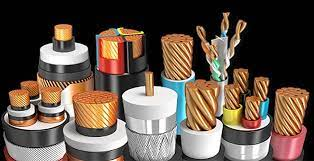
\includegraphics[scale=0.8]{Imagenes/Materiales_Conductores_01.jpg}
\end{figure}
\end{frame}
\begin{frame}
\frametitle{Materiales resistivos}
\begin{figure}
    \centering
    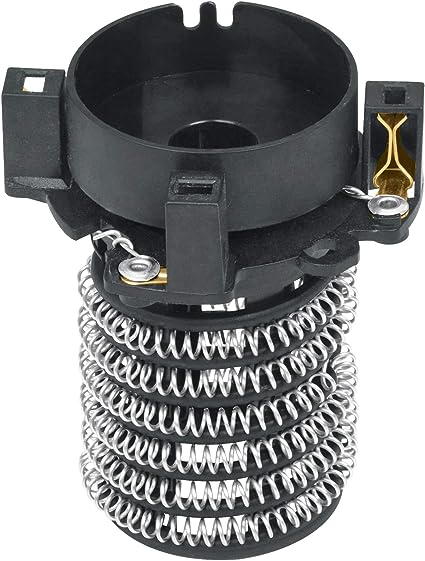
\includegraphics[scale=0.3]{Imagenes/Materiales_Conductores_02.jpg}
\end{figure}
\end{frame}
    
\subsection{Aislante}

\begin{frame}
\frametitle{Los aislantes}
Los materiales que no permiten que las partículas cargadas se muevan hacia otra región del material debido a una fuerza eléctrica, son llamados \textocolor{coolblack}{aislantes} por ejemplo, la madera.
\end{frame}

\subsection{Semiconductores}

\begin{frame}
\frametitle{Los materiales semiconductores}
Existen otros tipos de materiales cuyas propiedades son intermedias entre los conductores y aislantes: \pause  se llaman \textocolor{cornellred}{semiconductores}.
\end{frame}
\begin{frame}
\frametitle{Base de la electrónica}
Los materiales semiconductores con mayor utilidad en la electrónica son el silicio y el germanio.
\end{frame}

\section{Ley de Ohm}
\frame{\tableofcontents[currentsection, hideothersubsections]}
\subsection{La corriente}

\begin{frame}
\frametitle{La corriente eléctrica}
El flujo de las partículas cargadas es lo que se conoce como \textocolor{red}{corriente eléctrica}.
\end{frame}
\begin{frame}
\frametitle{La unidad de corriente}
La unidad de corriente eléctrica es el \textocolor{ao}{Ampere}, su símbolo es \si{\ampere}
\end{frame}
\begin{frame}
\frametitle{La corriente eléctrica}
Las partículas cargadas en una cierta dirección de un conductor chocan con los átomos, \pause produciendo una pérdida de energía que se manifiesta en forma de calor.
\end{frame}

\subsection{El voltaje}

\begin{frame}
\frametitle{El voltaje}
El \textocolor{cobalt}{voltaje}, \pause también conocido como \textocolor{amethyst}{diferencia de potencial eléctrico}.
\end{frame}
\begin{frame}
\frametitle{El voltaje}
El voltaje se puede ver como la \textocolor{cadmiumgreen}{fuerza impulsora} que permite que la corriente eléctrica fluya a través de los conductores.
\end{frame}
\begin{frame}
\frametitle{El voltaje}
Sus unidades son los \textocolor{brown(web)}{voltios} y su símbolo es \si{\volt}
\end{frame}

\subsection{La resistencia}

\begin{frame}
\frametitle{La resistencia eléctrica}
Una medida de \textocolor{blue}{oposición} que presentan las partículas cargadas al moverse libremente en una cierta dirección de un material conductor \pause es lo que se conoce como \textocolor{cerise}{resistencia eléctrica}.
\end{frame}
\begin{frame}
\frametitle{Unidades de la resistencia}
La unidad de la resistencia eléctrica es el \textocolor{carnelian}{Ohm}.
\\
\bigskip
\pause
Su símbolo es $\Omega$
\end{frame}

\subsection{Relación entre las variables}

\begin{frame}
\frametitle{La ley de Ohm}
La \textocolor{cornellred}{ley de Ohm} fue formulada por el físico alemán George Simon Ohm.
\end{frame}
\begin{frame}
\frametitle{La ley de Ohm}
En un circuito eléctrico describe la relación entre:
\pause
\setbeamercolor{item projected}{bg=corn,fg=black}
\setbeamertemplate{enumerate items}{%
\usebeamercolor[bg]{item projected}%
\raisebox{1.5pt}{\colorbox{bg}{\color{fg}\footnotesize\insertenumlabel}}%
}
\begin{enumerate}[<+->]
\item La corriente eléctrica $(I)$
\item La diferencia de potencial o voltaje $(V)$
\item La resistencia eléctrica $(R)$
\end{enumerate}
\end{frame}
\begin{frame}
\frametitle{La ley de Ohm}
La ley de Ohm se expresa matemáticamente mediante la siguiente ecuación:
\pause
\begin{align*}
V = I \, R
\end{align*}
\end{frame}
\begin{frame}
\frametitle{Ejercicios}
\setbeamercolor{item projected}{bg=denim,fg=white}
\setbeamertemplate{enumerate items}{%
\usebeamercolor[bg]{item projected}%
\raisebox{1.5pt}{\colorbox{bg}{\color{fg}\footnotesize\insertenumlabel}}%
}
\begin{enumerate}[<+->]
\item Un tostador eléctrico tiene una resistencia de \SI{30}{\ohm} cuando está caliente. ¿Cuál será la intensidad de la corriente que fluirá al conectarlo a una línea de \SI{120}{\volt}?
\seti
\end{enumerate}
\end{frame}
\begin{frame}
\frametitle{Ejercicios}
\setbeamercolor{item projected}{bg=denim,fg=white}
\setbeamertemplate{enumerate items}{%
\usebeamercolor[bg]{item projected}%
\raisebox{1.5pt}{\colorbox{bg}{\color{fg}\footnotesize\insertenumlabel}}%
}
\begin{enumerate}[<+->]
\conti
\item Determina la intensidad de la corriente eléctrica a través de una resistencia de \SI{50}{\ohm} al aplicarle una diferencia de potencial de \SI{120}{\volt}.
\seti
\end{enumerate}
\end{frame}
\begin{frame}
\frametitle{Ejercicios}
\setbeamercolor{item projected}{bg=denim,fg=white}
\setbeamertemplate{enumerate items}{%
\usebeamercolor[bg]{item projected}%
\raisebox{1.5pt}{\colorbox{bg}{\color{fg}\footnotesize\insertenumlabel}}%
}
\begin{enumerate}[<+->]
\conti
\item Un alambre conductor deja pasar \SI{7}{\ampere} al aplicarle una diferencia de potencial de \SI{110}{\volt}. ¿Cuál es su resistencia?
\end{enumerate}
\end{frame}

\section{Plantas generadoras de electricidad}
\frame{\tableofcontents[currentsection, hideothersubsections]}
\subsection{Tipos de plantas}


\begin{frame}
\frametitle{Generando la electricidad}
Existen diversos tipos de plantas generadoras de electricidad, cada una utilizando diferentes fuentes de energía y tecnologías.
\end{frame}
\begin{frame}
\frametitle{Centrales Térmicas}
\setbeamercolor{item projected}{bg=cadmiumgreen,fg=white}
\setbeamertemplate{enumerate items}{%
\usebeamercolor[bg]{item projected}%
\raisebox{1.5pt}{\colorbox{bg}{\color{fg}\footnotesize\insertenumlabel}}%
}
\begin{enumerate}[<+->]
\item Térmicas de Carbón: Queman carbón para generar vapor y accionar turbinas conectadas a generadores eléctricos.
\item Térmicas de Gas: Utilizan gas natural para producir vapor y generar electricidad.
\end{enumerate}
\end{frame}
\begin{frame}
\frametitle{Centrales Térmicas}
\vspace*{-1cm}
\begin{figure}
    \centering
    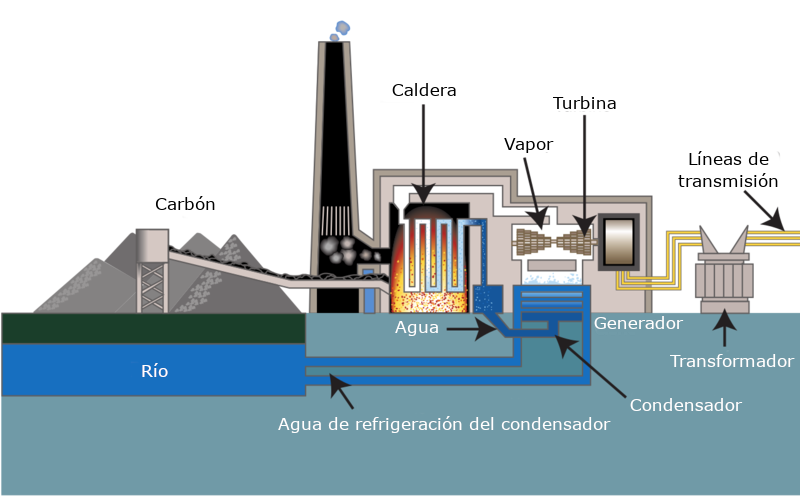
\includegraphics[scale=1.5]{Imagenes/Planta_Termica_01.png}
\end{figure}
\end{frame}
\begin{frame}
\frametitle{Centrales Hidroeléctricas}
Aprovechan la energía cinética del agua para hacer girar turbinas y generar electricidad.
\\
\bigskip
\pause
Pueden ser de embalse o de pasada.
\end{frame}
\begin{frame}
\frametitle{Centrales Hidroeléctrica}
\vspace*{-1cm}
\begin{figure}
    \centering
    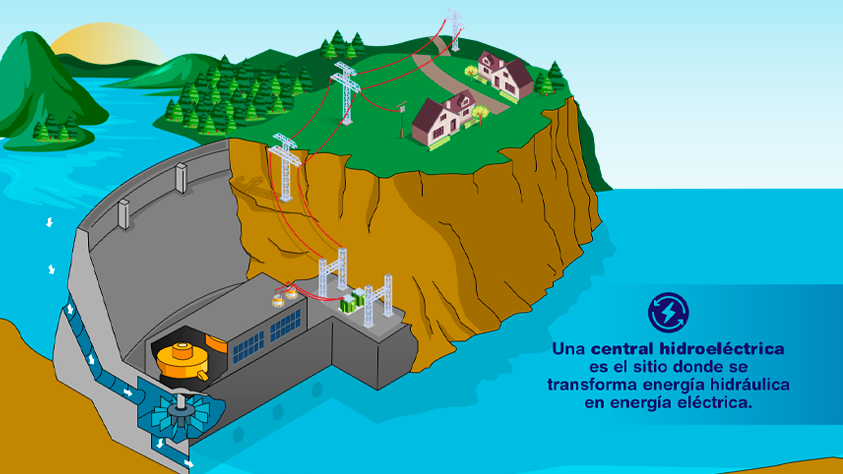
\includegraphics[scale=0.35]{Imagenes/Planta_Hidroelectrica.png}
\end{figure}
\end{frame}
\begin{frame}
\frametitle{Centrales Nucleares}
Utilizan la energía liberada en reacciones nucleares para generar calor, que a su vez produce vapor y activa turbinas.
\end{frame}
\begin{frame}
\frametitle{Centrales Nucleares}
\vspace*{-1cm}
\begin{figure}
    \centering
    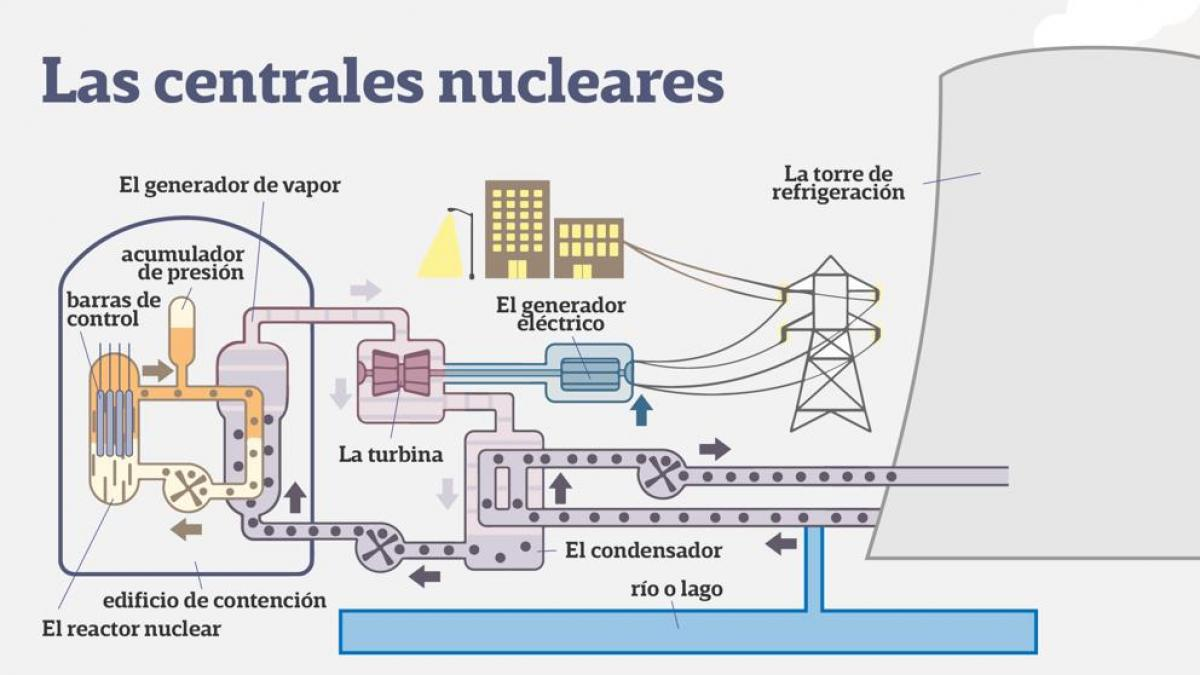
\includegraphics[scale=0.35]{Imagenes/Planta_Nuclear.jpeg}
\end{figure}
\end{frame}
\begin{frame}
\frametitle{Centrales Eólicas}
Convierten la energía cinética del viento en electricidad mediante aerogeneradores.
\end{frame}
\begin{frame}
\frametitle{Centrales Eólicas}
\vspace*{-1cm}
\begin{figure}
    \centering
    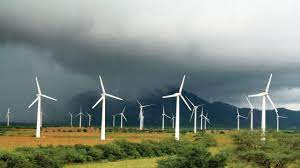
\includegraphics[scale=1]{Imagenes/Planta_Eolica_01.jpeg}
\end{figure}
\end{frame}
\begin{frame}
\frametitle{Centrales Eólicas}
\vspace*{-1cm}
\begin{figure}
    \centering
    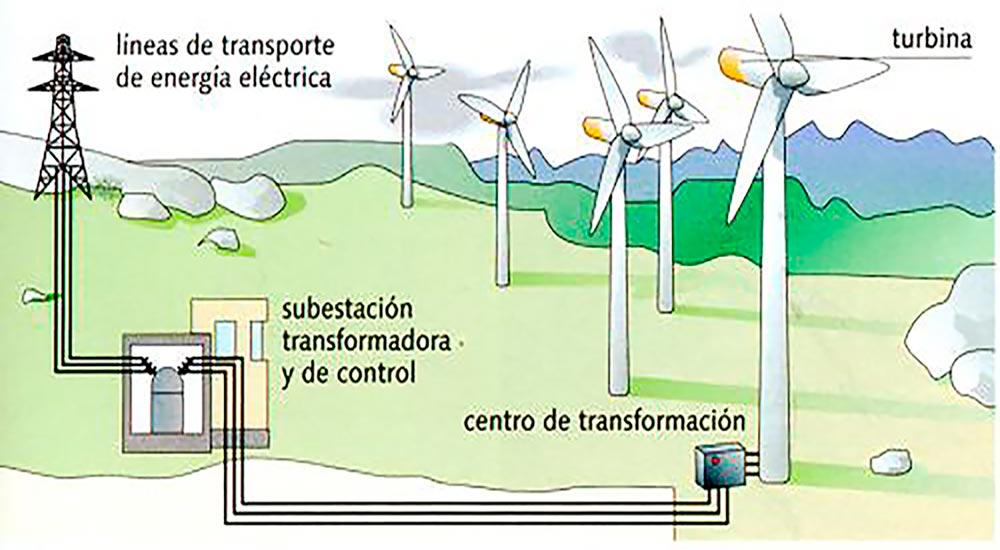
\includegraphics[scale=0.3]{Imagenes/Planta_Eolica_02.jpeg}
\end{figure}
\end{frame}
\begin{frame}
\frametitle{Centrales Solares}
Fotovoltaicas: Convierten la luz solar en electricidad utilizando celdas solares.
\end{frame}
\begin{frame}
\frametitle{Centrales Solares}
\vspace*{-1cm}
\begin{figure}
    \centering
    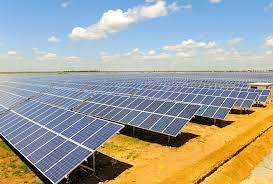
\includegraphics[scale=0.75]{Imagenes/Planta_Solar_01.jpeg}
\end{figure}
\end{frame}
\begin{frame}
\frametitle{Centrales Solares}
\vspace*{-1cm}
\begin{figure}
    \centering
    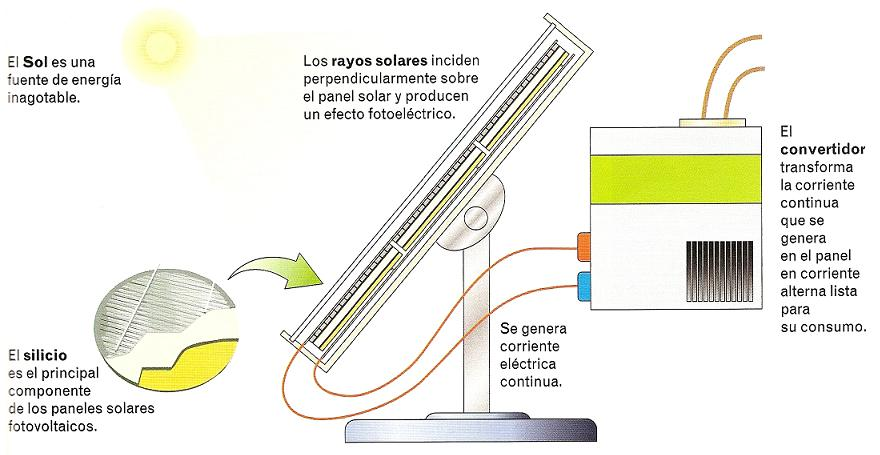
\includegraphics[scale=0.5]{Imagenes/Planta_Solar_02.jpeg}
\end{figure}
\end{frame}
\begin{frame}
\frametitle{Centrales de Biomasa}
Utilizan materiales orgánicos (madera, residuos agrícolas) para generar electricidad a través de procesos de combustión o gasificación.
\end{frame}
\begin{frame}
\frametitle{Centrales Geotérmicas}
Aprovechan el calor interno de la Tierra para generar vapor y accionar turbinas conectadas a generadores eléctricos.
\end{frame}
\begin{frame}
\frametitle{Centrales Geotérmicas}
\vspace*{-1cm}
\begin{figure}
\centering
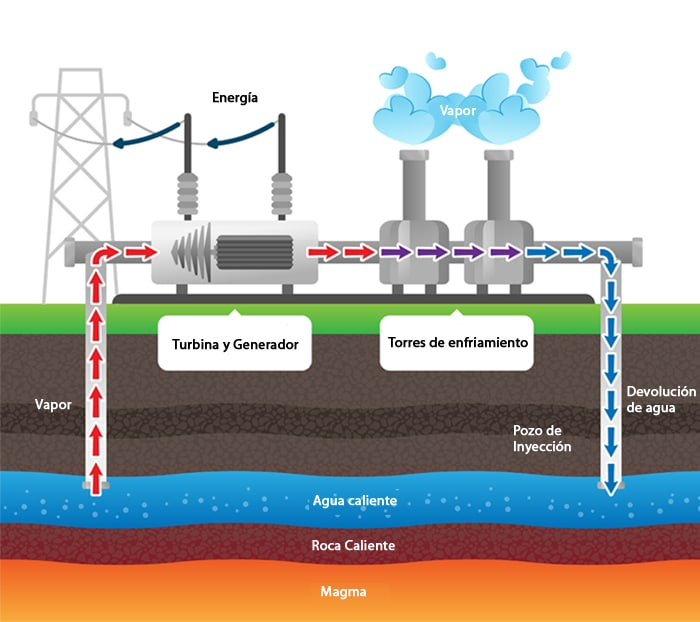
\includegraphics[scale=0.3]{Imagenes/Planta_Geotermica_01.jpg}
\end{figure}
\end{frame}

\section{Transmisión}
\frame[allowframebreaks]{\tableofcontents[currentsection, hideothersubsections]}
\subsection{Proceso de transimisión}

\begin{frame}
\frametitle{¿Para qué transmitir la electricidad?}
La \textocolor{ao}{transmisión de electricidad} desde las centrales generadoras hasta los puntos de consumo es una parte crítica de la infraestructura eléctrica.
\end{frame}
\begin{frame}
\frametitle{¿Qué se transmite?}
Este proceso implica el transporte eficiente de grandes cantidades de energía eléctrica a través de largas distancias.
\end{frame}

\subsection{Elementos de transmisión}

\begin{frame}
\frametitle{Torres de Transmisión}
Las líneas de transmisión aéreas utilizan torres para soportar los cables conductores.
\end{frame}
\begin{frame}
\frametitle{Torres de Transmisión}    
La altura y la disposición de estas torres se diseñan para maximizar la eficiencia de transmisión y minimizar las pérdidas.
\end{frame}
\begin{frame}
\frametitle{Torres de transmisión}
\vspace*{-1cm}
\begin{figure}
\centering
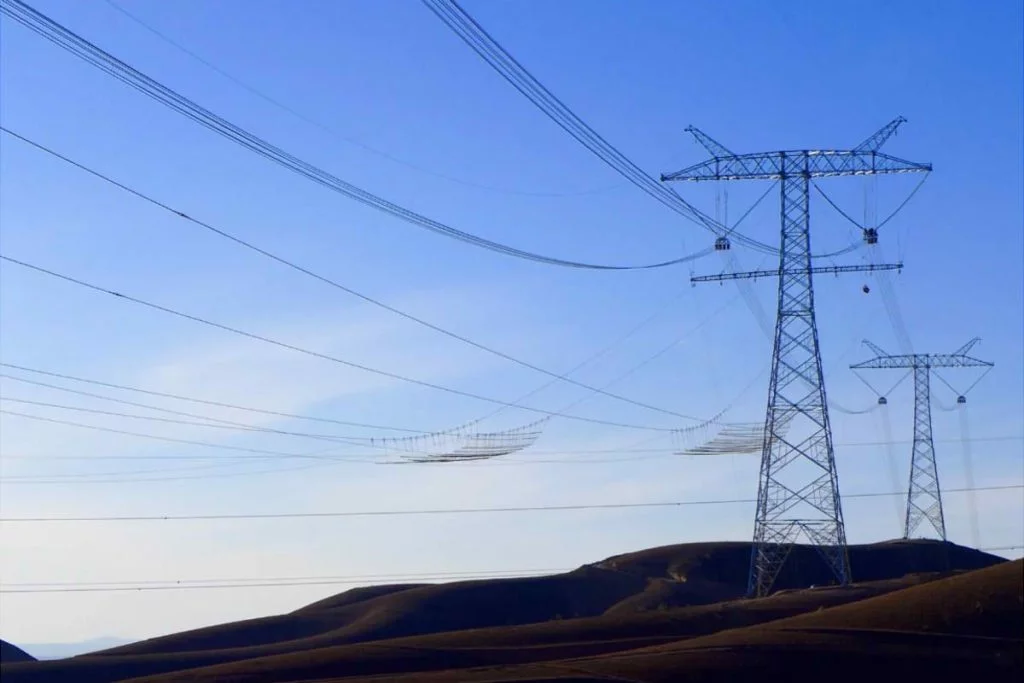
\includegraphics[scale=0.27]{Imagenes/Transmision_00.png}
\end{figure}
\end{frame}
\begin{frame}
\frametitle{Capacidad de Transmisión}
La \textocolor{byzantine}{capacidad de transmisión} de una línea se mide en volts-amperios (VA) \pause y se determina por la capacidad de carga de los conductores y la distancia entre las torres.
\end{frame}
\begin{frame}
\frametitle{Pérdidas de Transmisión}
A medida que la electricidad viaja a través de las líneas, \textocolor{coolblack}{se producen pérdidas} debido a la resistencia de los conductores y otros factores.
\end{frame}
\begin{frame}
\frametitle{Pérdidas de Transmisión}
Estas pérdidas se minimizan utilizando cables de mayor capacidad y optimizando el diseño de las líneas.
\end{frame}
\begin{frame}
\frametitle{La transmisión}
\vspace*{-1cm}
\begin{figure}
\centering
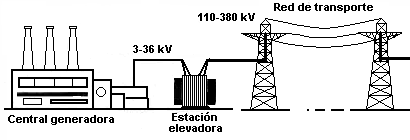
\includegraphics[scale=0.8]{Imagenes/Transmision_01.png}
\end{figure}
\end{frame}
\begin{frame}
\frametitle{La transmisión}
\vspace*{-1cm}
\begin{figure}
\centering
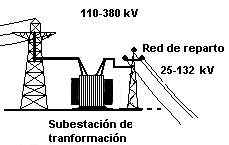
\includegraphics[scale=0.8]{Imagenes/Transmision_02.png}
\end{figure}
\end{frame}
\begin{frame}
\frametitle{La transmisión}
\vspace*{-1cm}
\begin{figure}
\centering
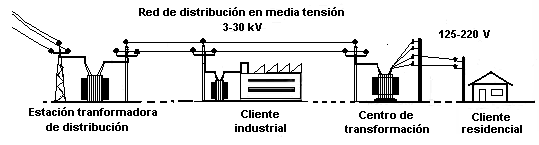
\includegraphics[scale=0.6]{Imagenes/Transmision_03.png}
\end{figure}
\end{frame}

\section{El generador eléctrico}
\frame[allowframebreaks]{\tableofcontents[currentsection, hideothersubsections]}
\subsection{Funcionamiento del generador}

\begin{frame}
\frametitle{Principio de operación}
Un \textocolor{byzantium}{generador de electricidad}, \pause es un dispositivo \textocolor{red}{que convierte energía mecánica} en \textocolor{cadmiumgreen}{energía eléctrica}.
\end{frame}
\begin{frame}
\frametitle{Principio de operación}
Este proceso se basa en el principio de la \textocolor{cobalt}{inducción electromagnética}, descubierto por Michael Faraday.
\end{frame}

\subsection{Partes de un generador}

\begin{frame}
\frametitle{Rotor}
Es la parte giratoria del generador.
\\
\bigskip
\pause
Puede consistir en un conjunto de bobinas conductoras o una estructura magnética.
\end{frame}
\begin{frame}
\frametitle{Rotor}
La rotación del rotor es esencial para generar un flujo magnético variable.
\end{frame}
\begin{frame}
\frametitle{Estator}
Es la parte estacionaria que rodea al rotor.
\\
\bigskip
\pause
El estator contiene un conjunto de bobinas conductoras.
\end{frame}
\begin{frame}
\frametitle{Estator}
Estas bobinas están dispuestas de manera que \textocolor{crimsonglory}{la variación del flujo magnético} generado por el rotor \pause \textocolor{darkmagenta}{induce corriente eléctrica} en las bobinas del estator.
\end{frame}
\begin{frame}
\frametitle{Campo Magnético}
Se crea mediante imanes permanentes o electroimanes.
\end{frame}
\begin{frame}
\frametitle{Campo Magnético}
El campo magnético puede ser fijo en el estator o girar con el rotor, dependiendo del diseño del generador.
\end{frame}
\begin{frame}
\frametitle{Generador eléctrico}
\vspace*{-1cm}
\begin{figure}
\centering
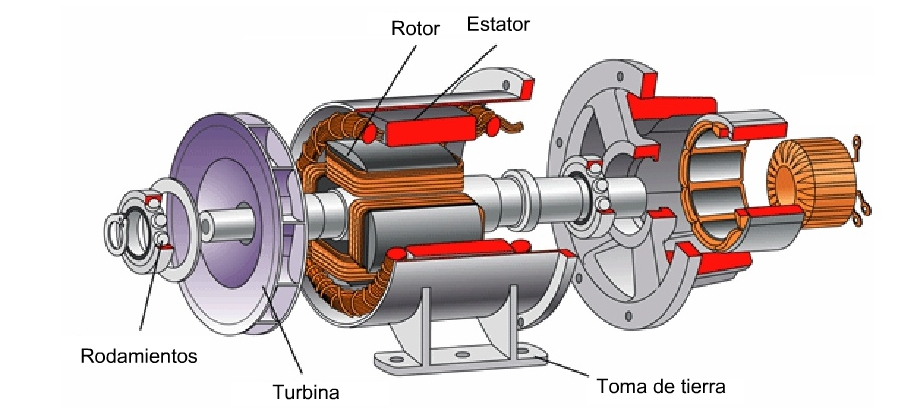
\includegraphics[scale=0.36]{Imagenes/Generador_01.jpg}
\end{figure}
\end{frame}

\subsection{Ley de inducción de Faraday}

\begin{frame}
\frametitle{Flujo Magnético Variable}
Cuando el rotor gira, se genera un \textocolor{darkscarlet}{flujo magnético variable} en el estator.
\end{frame}
\begin{frame}
\frametitle{Flujo Magnético Variable}
La variación del flujo magnético es esencial para inducir una corriente eléctrica.
\end{frame}
\begin{frame}
\frametitle{Inducción Electromagnética}
Según la \textocolor{debianred}{ley de Faraday de la inducción electromagnética}, \pause la \textocolor{dukeblue}{variación del flujo magnético} en una bobina \pause \textocolor{forestgreen(web)}{induce una corriente eléctrica} en esa bobina.
\end{frame}
\begin{frame}
\frametitle{Inducción Electromagnética}
Este proceso se aplica a las bobinas en el estator del generador.
\end{frame}
\begin{frame}
\frametitle{Producción de Corriente Alterna (AC)}
En el caso de un generador de corriente alterna, la corriente inducida en las bobinas del estator es inicialmente una corriente alterna.
\end{frame}
\begin{frame}
\frametitle{Producción de Corriente Alterna (AC)}
Esto se debe a que el flujo magnético varía con la rotación del rotor.
\end{frame}
\begin{frame}
\frametitle{Generadores de Corriente Continua (DC)}
En los generadores de corriente continua, la corriente alterna generada \textocolor{hanpurple}{se rectifica} mediante un conmutador para convertirla en corriente continua.
\end{frame}
\begin{frame}
\frametitle{Generadores de Corriente Continua (DC)}
El conmutador invierte la dirección de la corriente a medida que el rotor gira.
\end{frame}

\end{document}